\documentclass[addpoints]{exam}
\usepackage[utf8]{inputenc}
\usepackage[spanish]{babel}
\usepackage[T1]{fontenc}
\usepackage{charter}
\usepackage{amsmath}
\usepackage{amsfonts}
\usepackage{amssymb}
\usepackage{graphicx}
\usepackage{tikz}
\usepackage[outline]{contour} % glow around text
\usetikzlibrary{babel,calc,patterns,decorations.pathmorphing,decorations.markings,arrows.meta,shapes.geometric}
\usetikzlibrary{calc}
\tikzset{>=latex}
\contourlength{1.1pt}
\usepackage{tikz-3dplot}
\usepackage{multicol}
\usepackage{exam-randomizechoices}
\usepackage[left=1cm,right=1cm,top=2cm,bottom=2cm]{geometry}
\usepackage[font=small,labelfont={small,bf},margin=0.5cm,justification=justified]{caption}
\usepackage[font=small,labelfont={small,bf}]{subcaption}
\usepackage[italic,defaultmathsizes]{mathastext}
\usepackage{hyperref}
\usepackage{calculator}
\usepackage[breakable]{tcolorbox}
\usepackage{multirow}
\usepackage{tabularx}
\usepackage{cancel}
\usepackage{tipa}
\usepackage{enumerate}

%\pointpoints{punto}{puntos}
%\bonuspointpoints{punto extra}{puntos extra}

\renewcommand{\solutiontitle}{\textbf{Solución: }}
\renewcommand{\thequestion}{\bfseries\arabic{question}}

\newcommand{\sgn}{\mathop{\mathrm{sgn}}}
\newcommand{\diff}[0]{\mathrm{d}}
\newcommand{\fdiff}[2]{\frac{\mathrm{d} #1}{\mathrm{d} #2}}
\newcommand{\pdiff}[2]{\frac{\partial #1}{\partial #2}}
\newcommand{\fddiff}[2]{\frac{\mathrm{d^2} #1}{\mathrm{d} #2^2}}
\newcommand{\pddiff}[2]{\frac{\partial^2 #1}{\partial {#2}^2}}
\newcommand{\grado}[0]{^{\circ}}
\newcommand{\angulo}[3]{#1\grado \, #2' \, #3''}
\newcommand{\chel}[4]{^{#1}_{#2}\mbox{#3}^{#4}}
\newcommand{\valmed}[1]{\left\langle #1 \right\rangle}
\newcommand{\E}[1]{\times 10^{#1}}
\newcommand{\ver}[1]{\hat{\vec{#1}}}
\newcommand{\vecg}[1]{\boldsymbol{#1}}
\newcommand{\iu}{\mathrm{i}}
\newcommand{\norm}[1]{\left\vert\left\vert #1 \right\vert\right\vert}
\newcommand{\abs}[1]{\left\vert #1 \right\vert}
\newcommand{\tens}[1]{\mathbb{#1}}
\newcommand{\rr}{\mathbb{R}}
\newcommand{\un}[1]{\text{#1}}
\newcommand{\logoUNAHUR}{
\includegraphics[scale=0.35]{/home/shluna/UNAHUR/IAM/Apuntes/logo_unahur.png}}
\renewcommand{\arraystretch}{1.5}
\newcommand{\rta}{\textbf{Respuesta: }}
\newcommand{\rtas}{\textbf{Respuestas: }}
\newcommand{\ang}{110}
\newcommand{\angu}{-30}
\newcommand{\rad}{4}
\newcommand{\mg}{1}
\newcommand{\muc}{0.5}
\newcommand{\arc}[1]{{%
  \setbox9=\hbox{#1}%
  \ooalign{\resizebox{\wd9}{\height}{\texttoptiebar{\phantom{A}}}\cr#1}}}

  \colorlet{mydarkblue}{blue!40!black}
  \colorlet{myblue}{blue!30}
  \colorlet{myred}{red!65!black}
  \colorlet{vcol}{green!45!black}
  \colorlet{watercol}{blue!80!cyan!10!white}
  \colorlet{darkwatercol}{blue!80!cyan!80!black!30!white}
  \tikzstyle{water}=[draw=mydarkblue,top color=watercol!90,bottom color=watercol!90!black,middle color=watercol!50,shading angle=0]
  \tikzstyle{horizontal water}=[water,
    top color=watercol!90!black!90,bottom color=watercol!90!black!90,middle color=watercol!80,shading angle=0]
  \tikzstyle{dark water}=[draw=blue!20!black,top color=darkwatercol,bottom color=darkwatercol!80!black,middle color=darkwatercol!40,shading angle=0]
  \tikzstyle{vvec}=[->,very thick,vcol,line cap=round]
  \tikzstyle{force}=[->,myred,very thick,line cap=round]
  \tikzstyle{width}=[{Latex[length=3,width=3]}-{Latex[length=3,width=3]}]

\hypersetup{
%      draft,
   linktocpage=true,
    colorlinks=true,
    linkcolor=blue,
    citecolor=blue,
    filecolor=blue,      
    urlcolor=blue
}

\printanswers
\qformat{\textbf{Ejercicio \thequestion}\hfill}

\pagestyle{headandfoot}
\firstpageheader{Instituto de Tecnología e Ingeniería}{\logoUNAHUR}{Física III}
\firstpageheadrule
\runningheader{Segundo parcial}{\logoUNAHUR}{Física III}
\runningheadrule
\firstpagefooter{}{Página \thepage\ de \numpages}{}
\firstpagefootrule
\runningfooter{}{Página \thepage\ de \numpages}{}
\runningfootrule

\begin{document}

\renewcommand{\tablename}{Tabla}

\tdplotsetmaincoords{70}{110}

\begin{tcolorbox}[colback=white,arc=0mm,colframe=black]
    \begin{center}
        \Large\textbf{Física III -- Segundo parcial}
    \end{center}
\end{tcolorbox}

\vspace{11pt}

\textbf{Constantes utilizadas:} $\epsilon_0 = 8.85 \E{-12} \, \dfrac{\text{C}^2}{\text{N} \, \text{m}^2}$, $\mu_0 = 4 \, \pi \, \E{-7} \, \dfrac{\text{T} \, \text{m}}{\text{A}}$.

\vspace{11pt}

\begin{tcolorbox}[colback=black!5!white,arc=0mm,breakable,pad at break*=1mm,colframe=black!25!white,title=\textbf{\textcolor{black}{Ecuación de ondas}}]
    La ecuación de onda describe la propagación de una perturbación $\psi$ que se propaga en el espacio y el tiempo $t$. Si la propagación ocurre en la dirección $x$, esta ecuación toma la forma:
    \begin{equation}
        \label{ec:ec_de_onda_x}
        \pddiff{\psi}{t} = v^2 \, \pddiff{\psi}{x},
    \end{equation} donde $v$ es la rapidez (constante) con la que se propaga la perturbación, la cual depende de las propiedades del medio. En este caso $\psi = \psi (x,t)$.

    \vspace{11pt}

    Para el caso de una perturbación que se propaga en el espacio, la ecuación de onda toma la forma:
    \begin{equation}
        \label{ec:ec_de_onda_3D}
        \pddiff{\psi}{t} = v^2 \, \nabla^2 \psi,
    \end{equation} donde $\psi = \psi(\vec{r},t) = \psi (x,y,z,t)$.
\end{tcolorbox}

\vspace{11pt}

\begin{questions}
    
    \question Verificar que las siguientes expresiones de las intensidades de los campos eléctrico ($E$) y magnético ($B$) satisfacen las ecuaciones de onda correspondientes.
    \begin{align*}
        E &= E_0 \cos \left(k \, x - \omega \, t\right), \\
        B &= B_0 \cos \left(k \, x - \omega \, t\right).
    \end{align*} Además, conteste las siguientes preguntas:
    \begin{parts}
        \part ¿Con qué rapidez se propagan las ondas electromagnéticas?
        \part ¿Cuál es la relación entre las amplitudes de los campos eléctrico y magnético?
        \part ¿Pueden las expresiones de $E$ y de $B$ reescribirse como funciones del argumento $x - c \, t$? ¿Por qué?
        \part ¿En qué dirección se propagan $E$ y $B$?
    \end{parts}

    \question Suponga que usted está ubicado a 180 m de un transmisor de radio.
    \begin{parts}
        \part ¿A cuántas longitudes de onda del transmisor de radio si la estación se llama 1150 AM? (Las frecuencias de la banda AM están en kHz).
        \part ¿Qué pasaría si la estación fuera de 98.1 FM? (Las frecuencias de la banda FM están en MHz).
    \end{parts}

    \question Un pulso de radar vuelve al receptor después de un tiempo total de recorrido de $4.0 \E{-4}$ s. ¿A qué distancia está el objeto que reflejó la onda?

    \question El anuncio de una noticia importante se transmite por ondas de radio a un auditorio de personas sentadas junto a sus aparatos de radio a 100 km de la estación, y por ondas sonoras a las personas que están sentadas en la sal de noticias, a 3m del locutor. ¿Quién recibe la noticia primero? Justifique su respuesta.

    \textbf{Dato:} Suponga que la velocidad del sonido es de $343 \, \dfrac{\text{m}}{\text{s}}$.

    \question Una onda electromagnética en el vacío tiene una amplitud de campo eléctrico de $220 \, \dfrac{\text{V}}{\text{m}}$. Calcule la amplitud del campo magnético correspondientes.

    \question La Figura~\ref{fig:ondaEM} muestra una onda electromagnética senoidal plana que se propaga en la dirección $x$. Suponga que la longitud de onda es de 50 m, y que el campo eléctrico vibra en el plano $xy$ con un amplitud de $22 \, \frac{\text{V}}{\text{m}}$. Calcule
    \begin{parts}
        \part la frecuencia de la onda y 
        \part la magnitud y dirección de $\vec{B}$ cuando el campo eléctrico tiene su valor máximo en la dirección negativa de las $y$.
        \part Escriba una expresión para $\vec{B}$ utilizando el vector unitario correcto, con valores numéricos para $\vec{B}$, $k$ y $\omega$, y con su magnitud de la forma: $$B = B_0 \cos \left(k \, x - \omega \, t\right)$$
    \end{parts}

    \begin{figure}[ht]
        \centering
        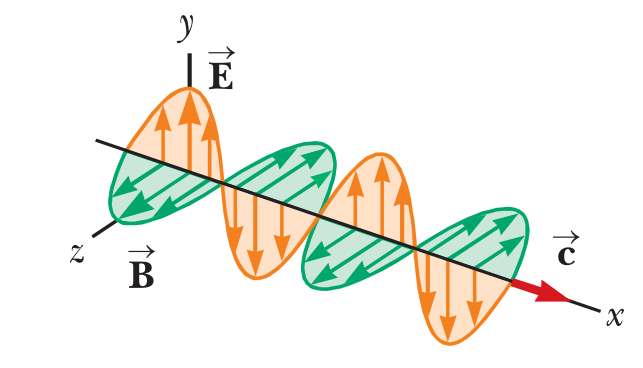
\includegraphics[scale=0.4]{ondaEM.png}
        \caption[Onda electromagnética]{Esquema de una onda electromagnética.}
        \label{fig:ondaEM}
    \end{figure}

    \question Escriba las expresiones para los campos eléctrico y magnético de una onda electromagnética senoidal plana que tiene una frecuencia de 3 Ghz y que se desplaza en la dirección positiva de las $x$. La amplitud del campo eléctrico es de $300 \, \frac{\text{V}}{\text{m}}$.

    \question En unidades del SI, el campo eléctrico de una onda electromagnética se describe por $$ E_y = 100 \, \frac{\text{N}}{\text{C}} \sen \left(1.0 \E{7} \, x - \omega \, t\right)$$ Determine:
    \begin{parts}
        \part la amplitud de las oscilaciones del campo magnético correspondientes,
        \part la longitud de onda $\lambda$ y 
        \part la frecuencia $f$.
    \end{parts}

    \question ¿Cuánta energía electromagnética por metro cúbico contiene la luz solar, si la intensidad de esta en la superficie de la Tierra en un día despejado es de $1000 \, \dfrac{\text{W}}{\text{m}^2}$.

    \question ¿Cuál es la magnitud promedio del vector de Poynting a 8 km de un transmisor de radio que difunde de manera isotrópica con una potencia promedio de 250 kW? Calcule también las intensidades máximas del campo eléctrico y del campo magnético.

    \question Una fuente de luz monocromática emite 100 W de energía electromagnética de manera uniforme en todas direcciones.
    \begin{parts}
        \part Calcule la densidad de energía del campo eléctrico promedio a 1 m de la fuente.
        \part Calcule la densidad de energía del campo magnético promedio a la misma distancia de la fuente.
        \part Determine la intensidad de la onda en esta ubicación.
    \end{parts}

    \begin{figure}
        \centering
        \begin{subfigure}{0.45\textwidth}
            \centering
            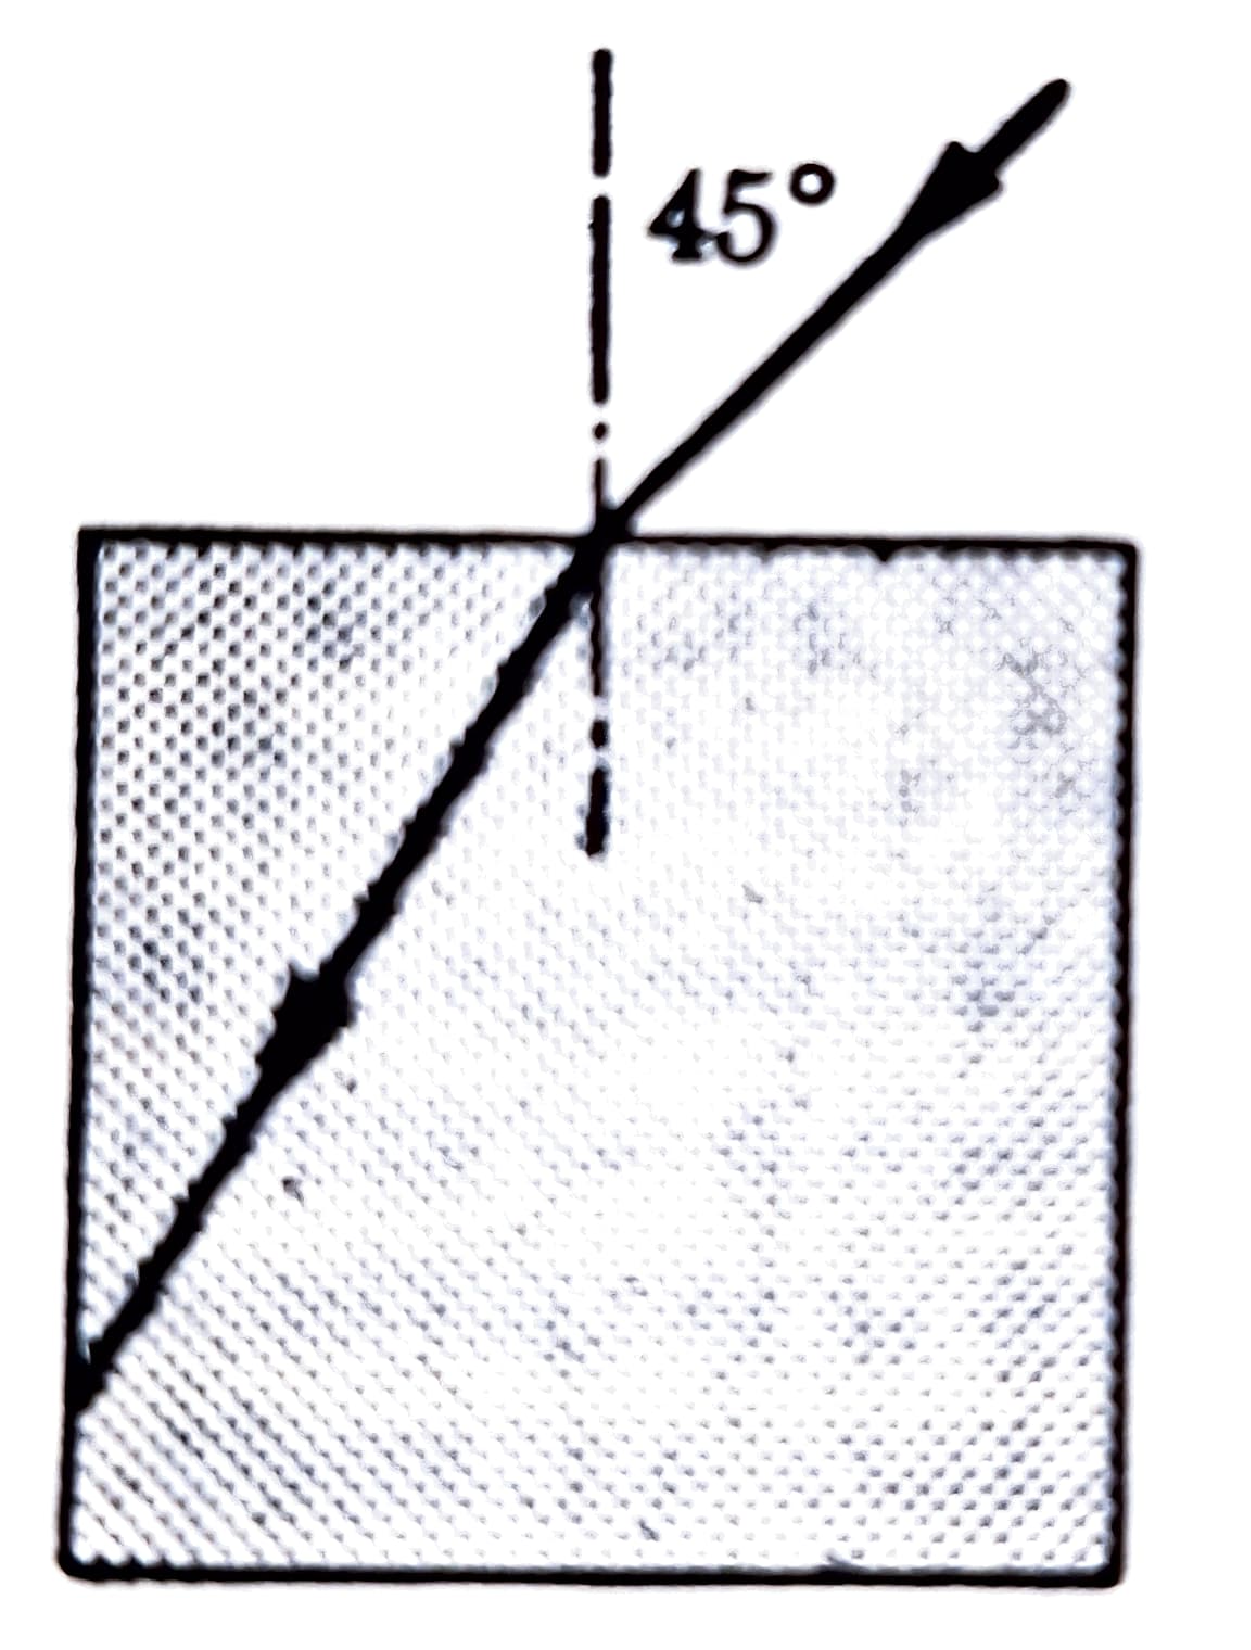
\includegraphics[scale=0.15]{reflexiontotal.pdf}
            \caption{ }
            \label{fig:reflexiontotal}
        \end{subfigure}
        ~
        \begin{subfigure}{0.45\textwidth}
            \centering
            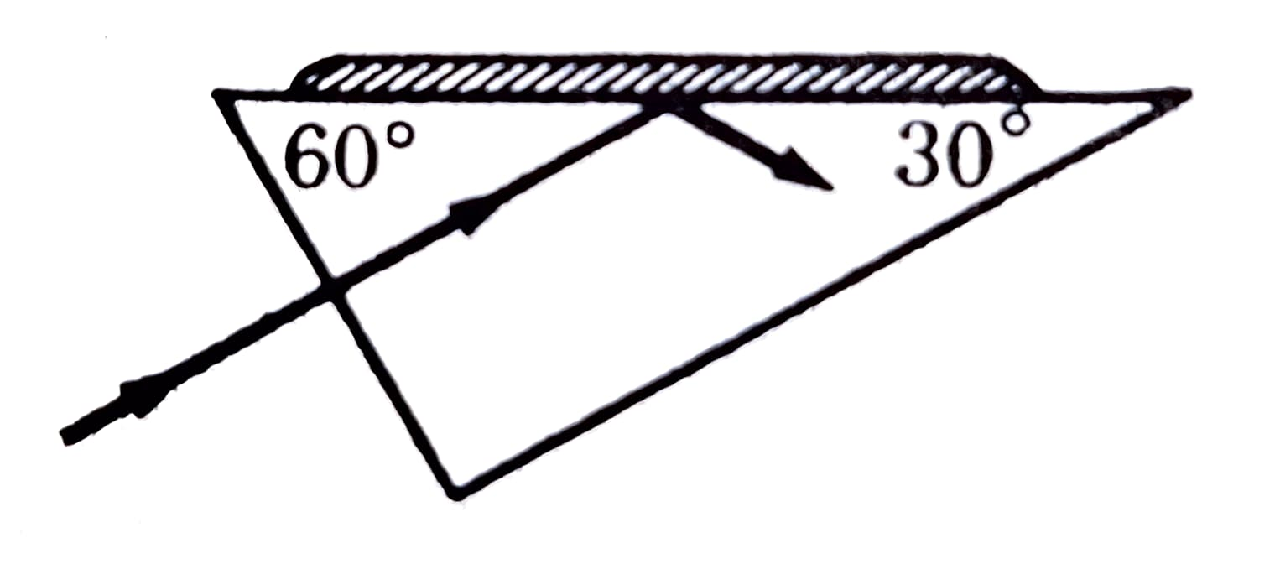
\includegraphics[scale=0.3]{refraccion.pdf}
            \caption{}
            \label{fig:refraccion}
        \end{subfigure}
        \caption{ }
    \end{figure}

    \question Un rayo de luz incide con un ángulo de $45\grado$ sobre la superficie superior de un cubo de vidrio como el de la Figura~\ref{fig:reflexiontotal}. El índice de refracción del vidrio es de $1.414$. ¿Se refleja totalmente el rayo en la cara vertical?

    \question Un rayo de luz incide normalmente sobre la cara menor de un prisma cuyos ángulos son $30\grado - 60\grado - 90\grado$, como el de la Figura~\ref{fig:refraccion}. Se coloca una gota de líquido sobre la hipotenusa del prisma. Si el índice de refracción del prisma es de $1.5$, calcule el índice máximo de refracción que puede tener el líquido si la luz ha de reflejarse totalmente.

    \question Dos orificios separados por $0.5$ mm están iluminados por uun haz de láser helio-neón que emite luz monocromática de longitud de onda de $0.6328 \E{-6}$ m. Una pantalla está ubicada 5 m detrás de aquella que contiene a los orificios. ¿Cuál es la separación de las franjas de interferencia sobre la pantalla?

\end{questions}

\end{document}